%===============================================================================
\appendix

%===============================================================================

\section{Appendix: Milestone plan}
\label{appendix:milestone_plan}

\begin{sidewaysfigure}[ht]
    \centering
    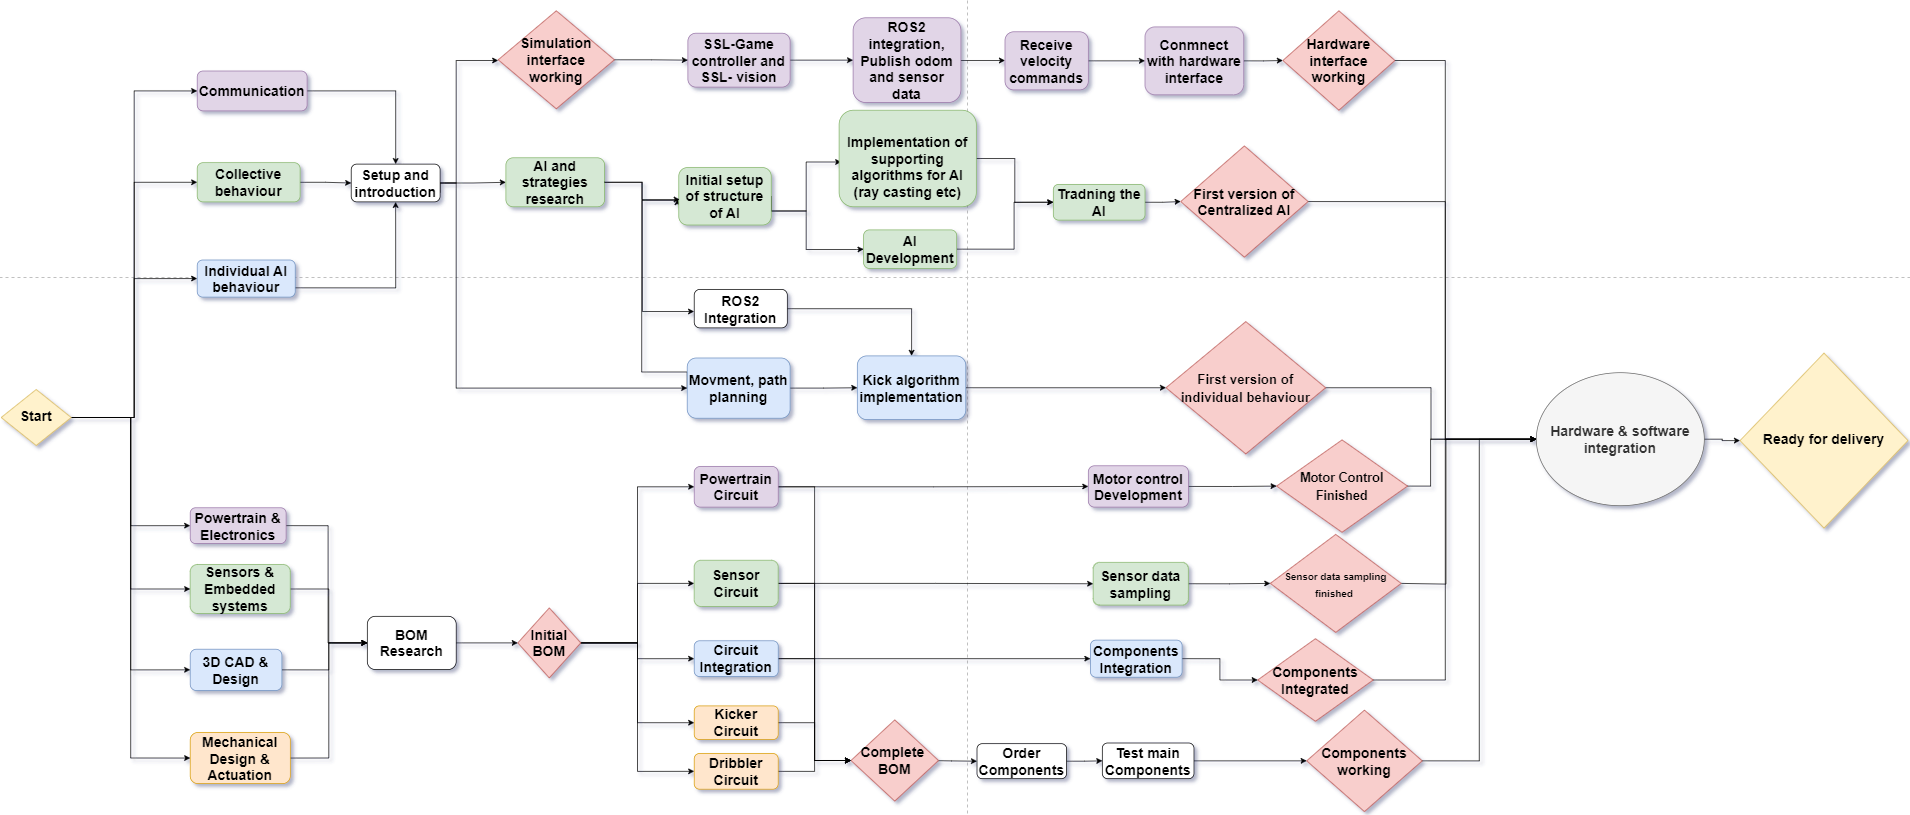
\includegraphics[width=\linewidth]{images/MileStone.png}
    \caption{The milestone plan for the project.}
    \label{fig:mile_stone} 
\end{sidewaysfigure}

%===============================================================================

\section{Appendix: Bill of Materials}
\label{appendix:bom}

\begin{table}[H]
    \centering
    \renewcommand{\arraystretch}{1.2} % Adjust row height
    \large % Increase text size
    \begin{tabularx}{\textwidth}{|X|X|X|X|} \hline
         \textbf{Component} & \textbf{Features} & \textbf{Purpose} & \textbf{Price (SEK)}  \\ \hline
         DF45L024048-A-Brushless \ac{dc} Motor & Good torque, built-in sensors, small footprint & Motors connected to the wheels to drive the robot in all directions & $3273.6\ (818.4 \times 4)$ \\ \hline
         Hobbywing FPV XRotor 3110 900KV & Supports very high \ac{rpm} needed for the dribbler & Part of the dribbler system that adds spin to the ball to increase control & $175.2$\\ \hline
         Aerostar 30A RVS G2 32bit \ac{esc} & PWM-based \ac{esc} to control motor speed & To control the motors & $736\ (147.2 \cdot4)$\\ \hline
         Arduino Nano & Samples output current of each phase, closed-loop PID system to regulate PWM signal & Regulate the PWM signal & $1196\ (299 \cdot4)$ \\ \hline
         Hall effect current sensor & Hall effect current sensor to measure the current of each phase in the \ac{esc} & Measure phase current &$576 (48\cdot4\cdot3)$\\ \hline
         ESP32-WROVER-IE & Low power consumption, Wi-Fi communication & A \ac{mcu} to collect sensory information, communicate with the external computer, and control the motors & Sponsored by \ac{mdu}\\ \hline
         Raspberry Pi 4 Model B/8GB & Multiple connection ports, 8GB \ac{ram}, low power mode & A \ac{mcu} to handle camera input, run Nav2, and send motor instructions to the ESP32 & $979$\\ \hline
         6s 1300mAh-120C-GNB HV XT60 & Sufficient energy capacity, low price, small footprint, low weight & Provide voltage and current to all sensors and actuators & $351.2$\\ \hline
         LT3750 & Capacitor charging controller for kicker, adjustable output voltage, integrated security control & Charges capacitors to sufficient levels (up to 300V) for passing and shooting & $146.9$\\ \hline
         iC-PX2604 and PX01S 26-30 & Optical encoder and wheel for accurate wheel orientation readings & Uses slits in the encoder wheel to read position & $897.6\ (224.4 \cdot4)$\\ \hline
         WSEN-ISDS 6 Axis \ac{imu} & Reads up to $\pm 16g$ and $\pm 2000$ \ac{dps} &  & Sponsored by Würth Electronics\\ \hline
         Raspberry Pi Camera Module 3 & Commonly used in \ac{ssl} modules for object detection &  & $369$\\ \hline
         LEDEX 195207-228 & Solenoid for the kicker &  & Sponsored by \ac{mdu}\\ \hline
    \end{tabularx}
    \caption{The preliminary \acl{bom} for the project.}
    \label{tab:bom}
\end{table}

%===============================================================================